\documentclass[convert]{standalone}

\usepackage{tikz}
\usepackage{graphicx}
\pagestyle{empty}

% INT_AY22_L28-Fig13_E_field_vs_t_graph.png

\begin{document}
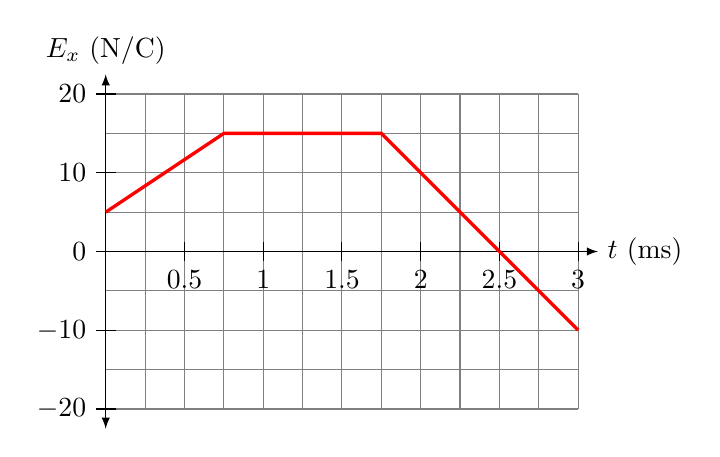
\begin{tikzpicture}[> = latex]

	% Grid
	
	\draw [thin, gray, step = 0.5 cm] (0, -2) grid (6, 2);

	% Axes
	
	\draw [<->] (0, 2.25) node [above] {$E_x$ (N/C)} -- (0, -2.25);
	\draw [->] (0, 0) -- (6.25, 0) node [right] {$t$ (ms)};
	
	% Axis labels + tick marks
	
	\foreach \x in {0.5, 1, ..., 3}
		\draw (2 * \x, 0.125) -- (2 * \x, -0.125) node [below] {$\x$};
	
	\foreach \y in {-20, -10, ..., 20}
		\draw (0.125, 0.1 * \y) -- (-0.125, 0.1 * \y) node [left] {$\y$};
		
	% E_x vs. t curve
	
	\draw [very thick, red] (0, 0.5) -- (1.5, 1.5) -- (3.5, 1.5) -- (6, -1);
	
\end{tikzpicture}
\end{document}